\clearpage
\chapter{Results}\label{sec:results}
%Unblinded result data no excess over the standard model prediction.
Exclusion limit plot.
Results

 \begin{figure}[h!]
   \caption{Cutflow histogram of MS15GeV-ct10mm point. Left plot is for region A, whereas the right plot is for region D}
   \label{fig:ABmethod}
   \centering
   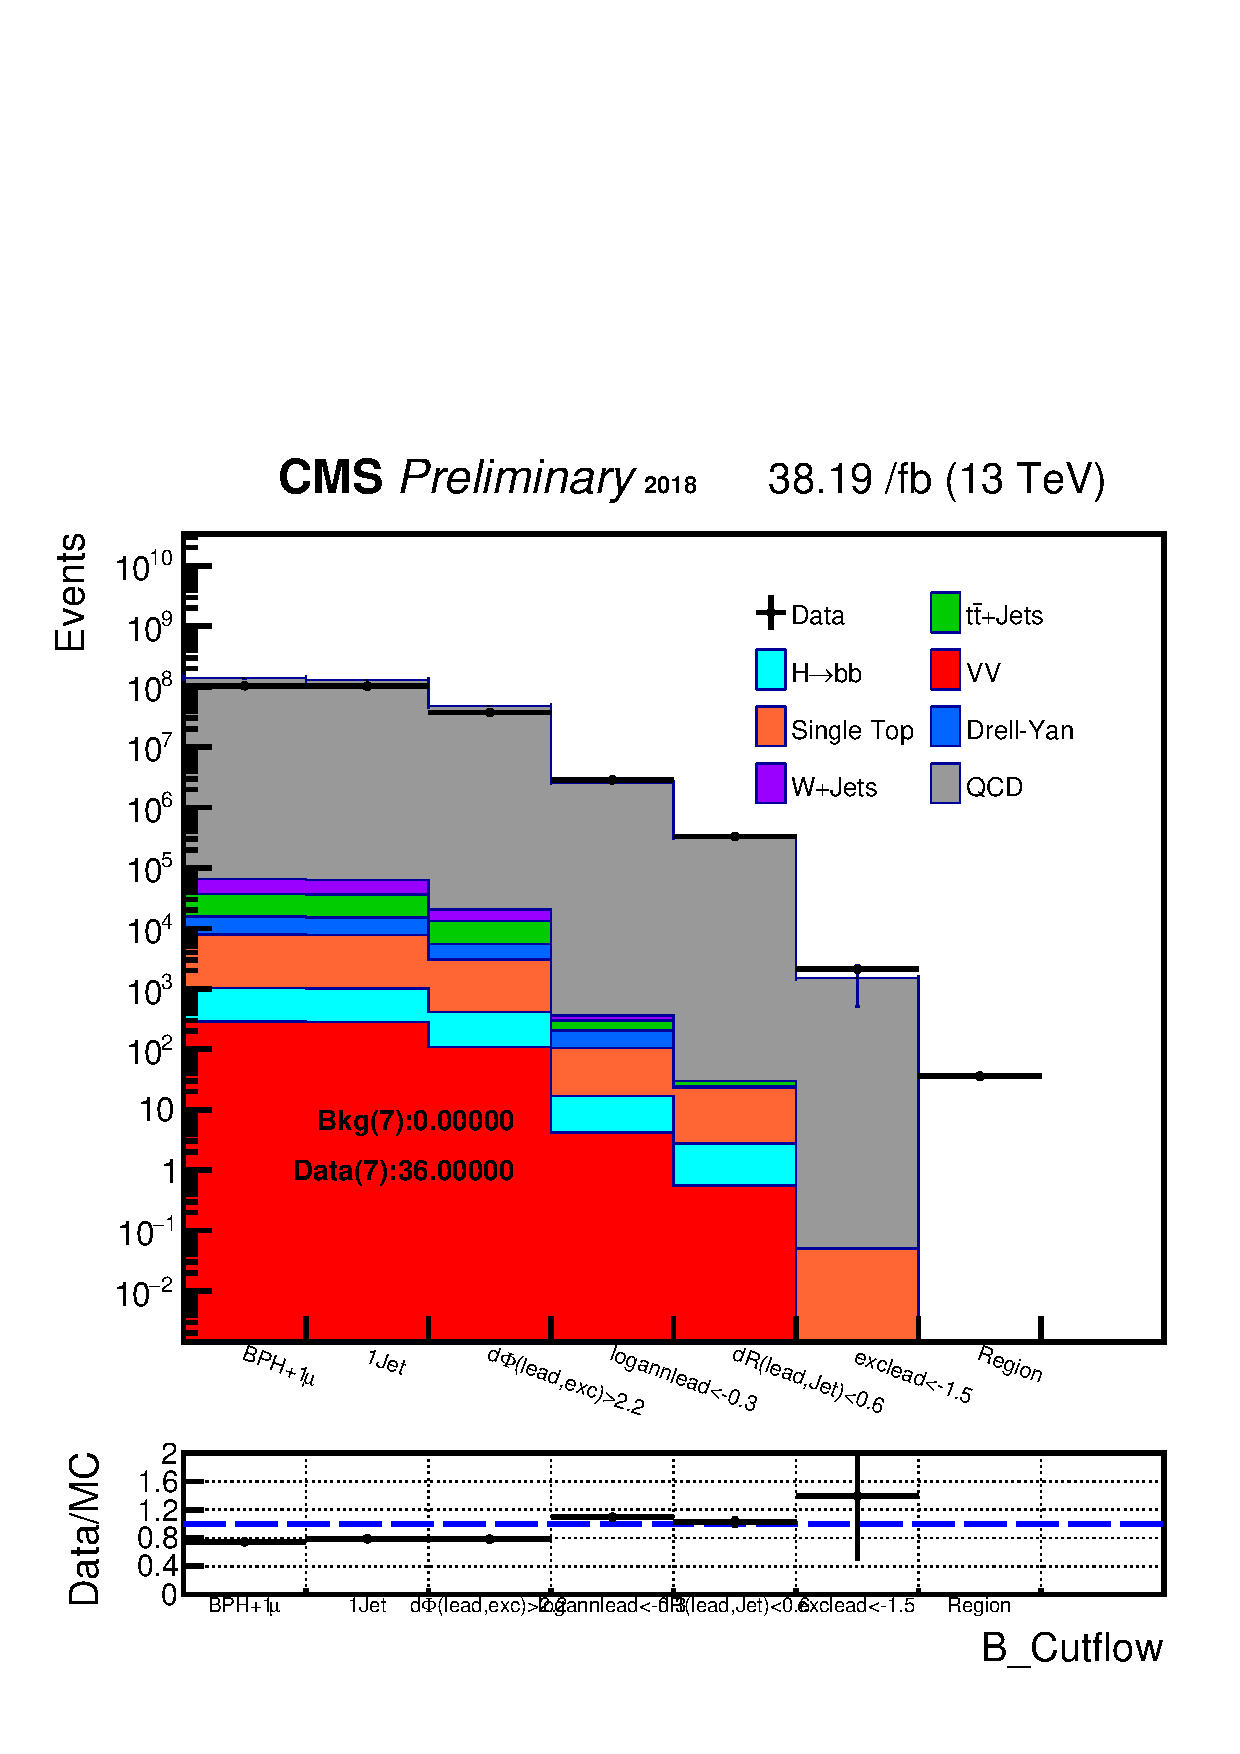
\includegraphics[width=0.47\linewidth]{figs/Data_log_CutflAnalysisNote_MS-15_ctauS-10_B_Cutflow.pdf}
   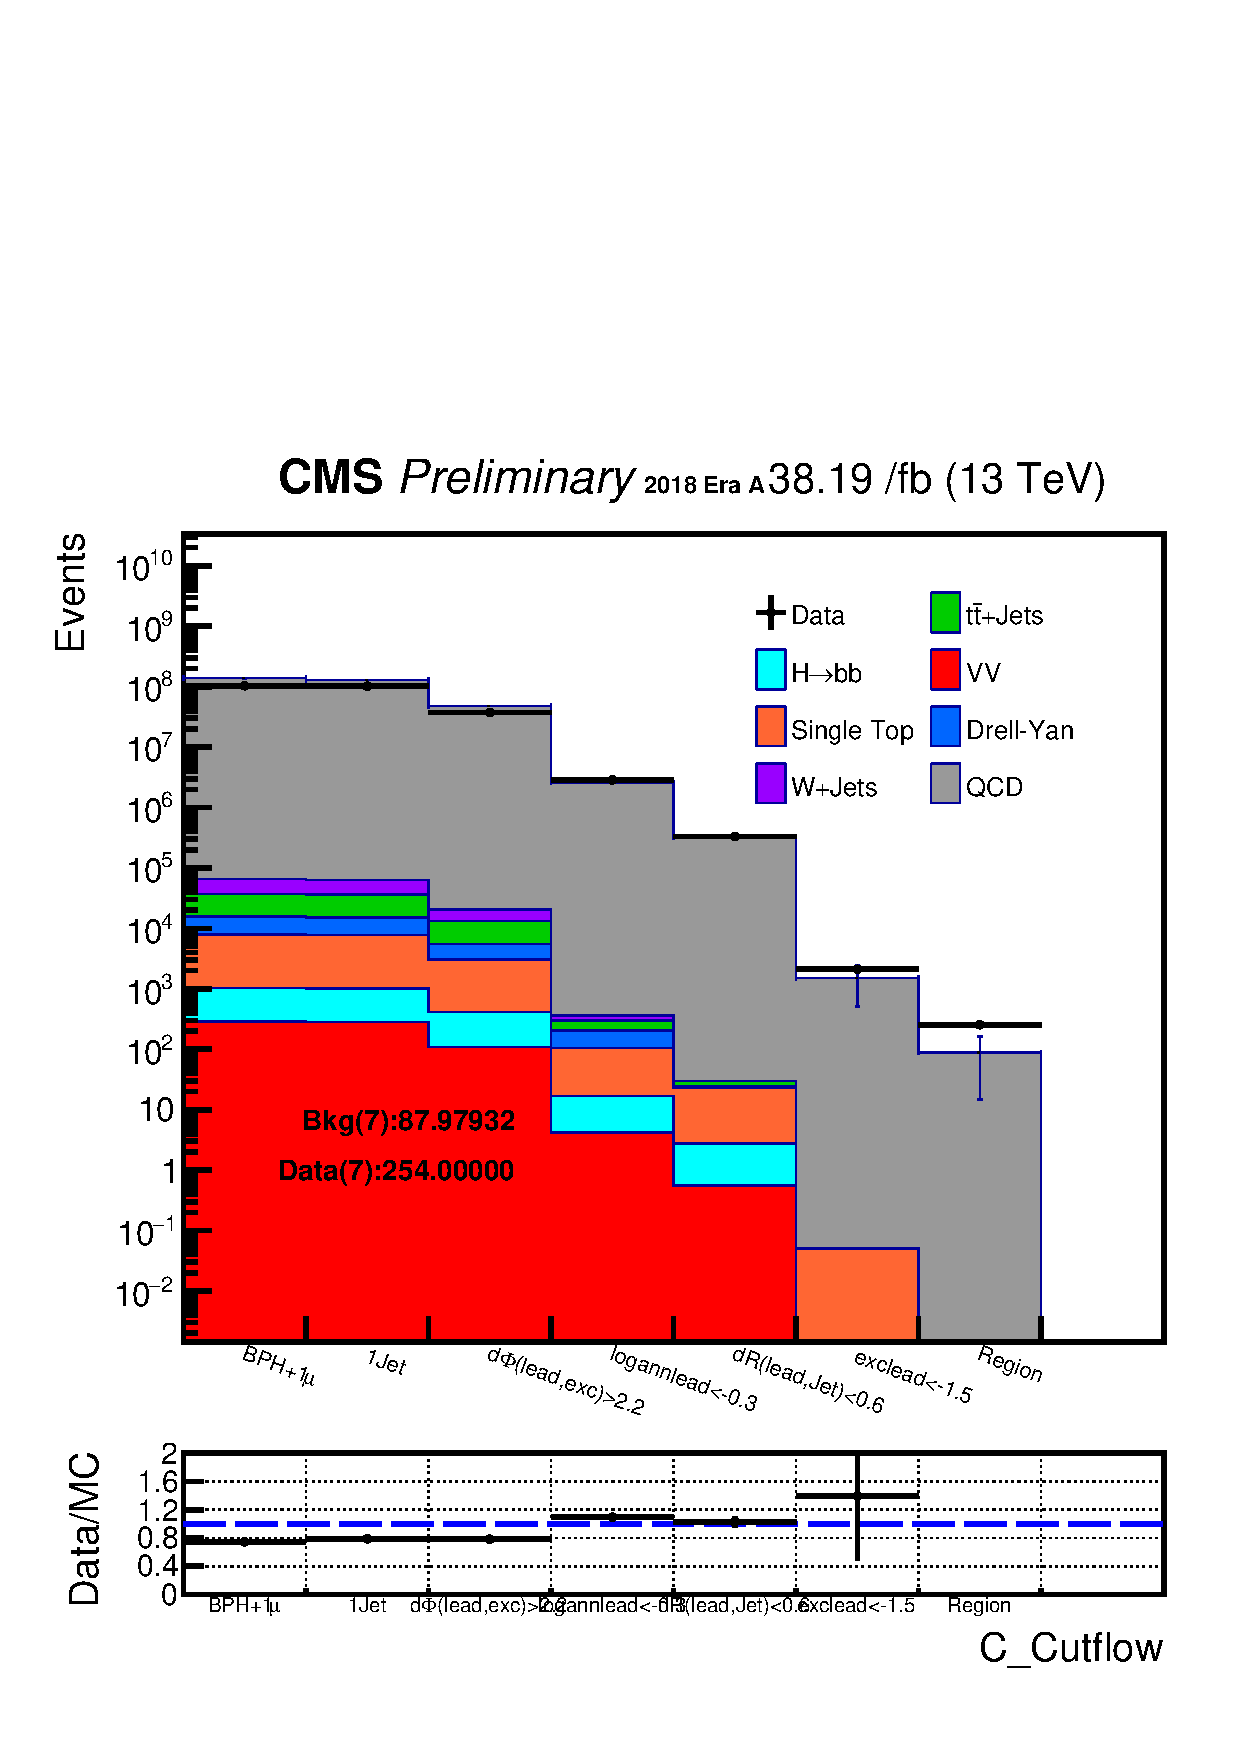
\includegraphics[width=0.47\linewidth]{figs/Data_log_CutflAnalysisNote_MS-15_ctauS-10_C_Cutflow.pdf}
   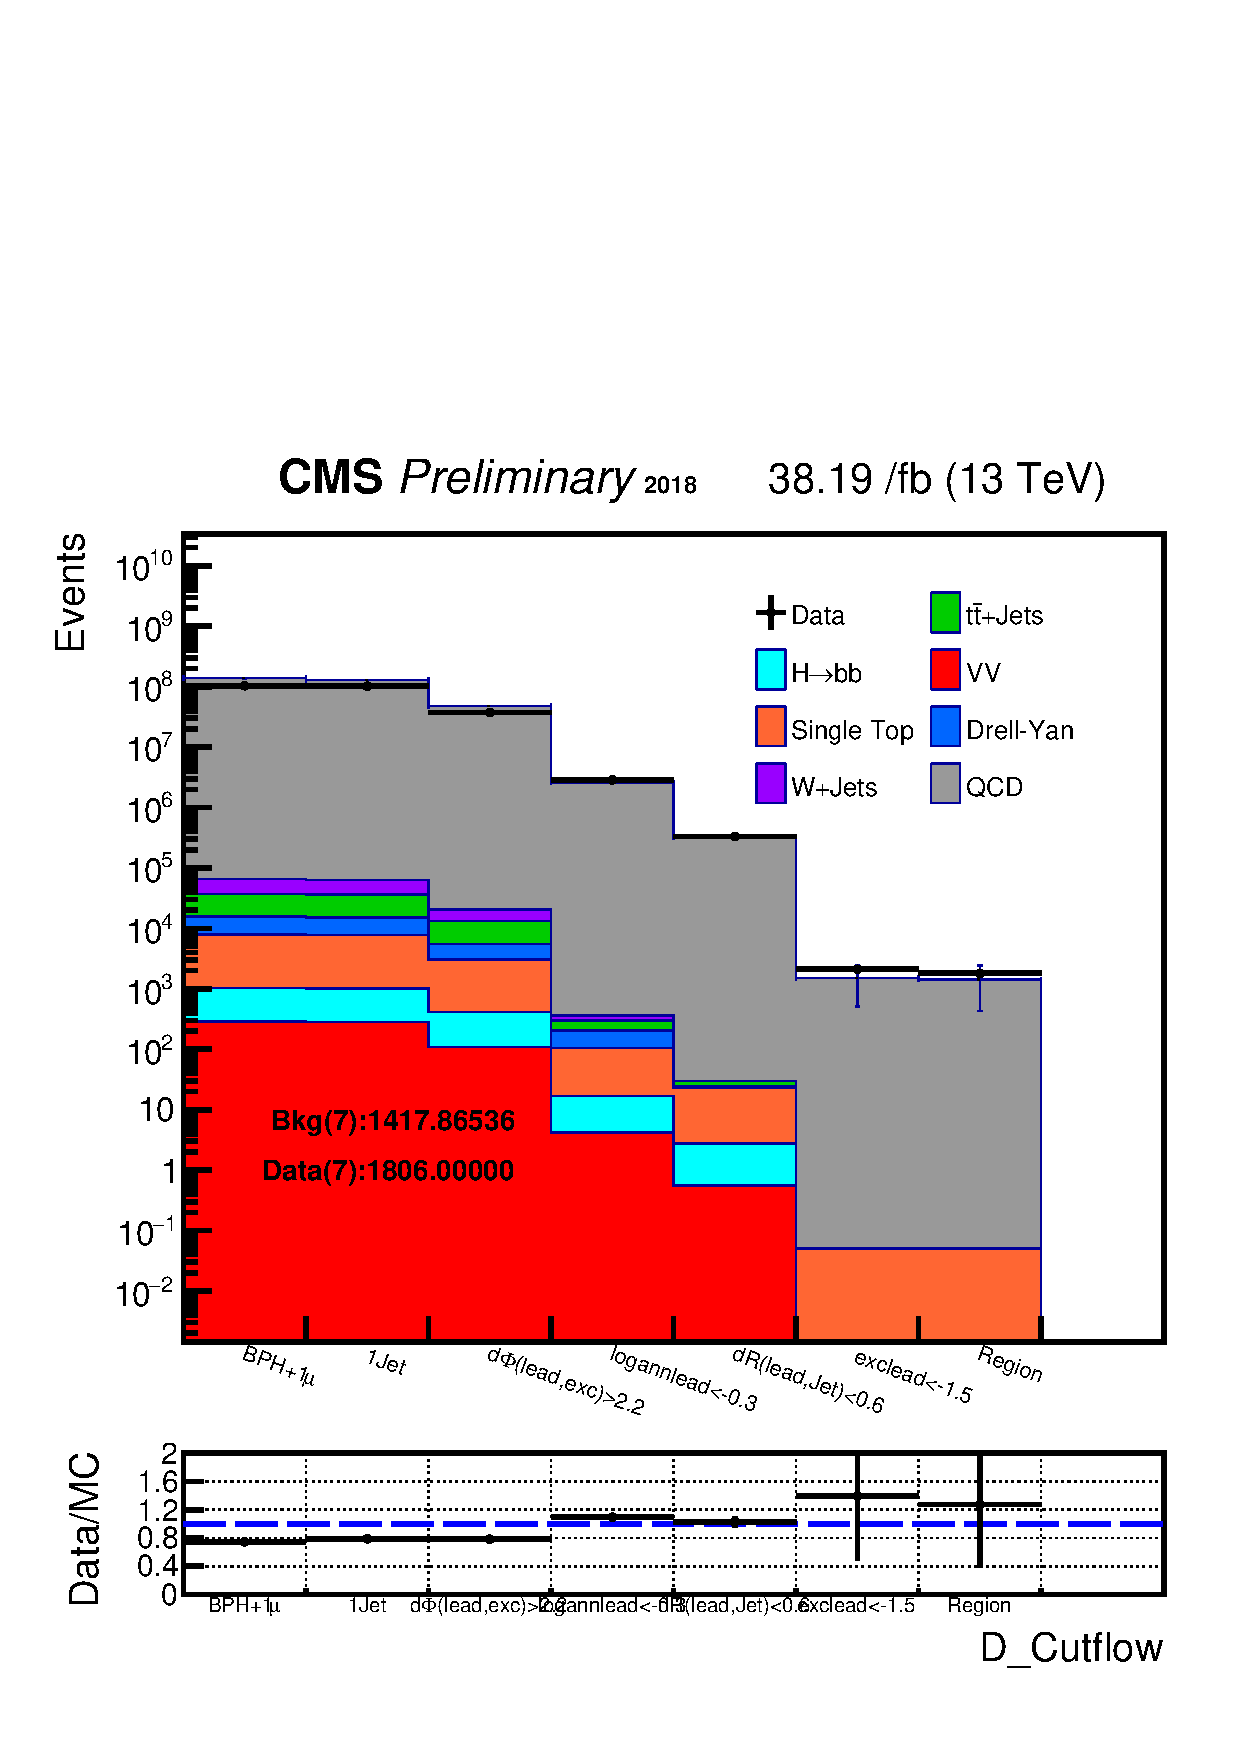
\includegraphics[width=0.47\linewidth]{figs/Data_log_CutflAnalysisNote_MS-15_ctauS-10_D_Cutflow.pdf}
 \end{figure}


\begin{figure}[h!]
   \caption{Current Preliminary limit plots}
   \label{fig:Limit}
   \centering
   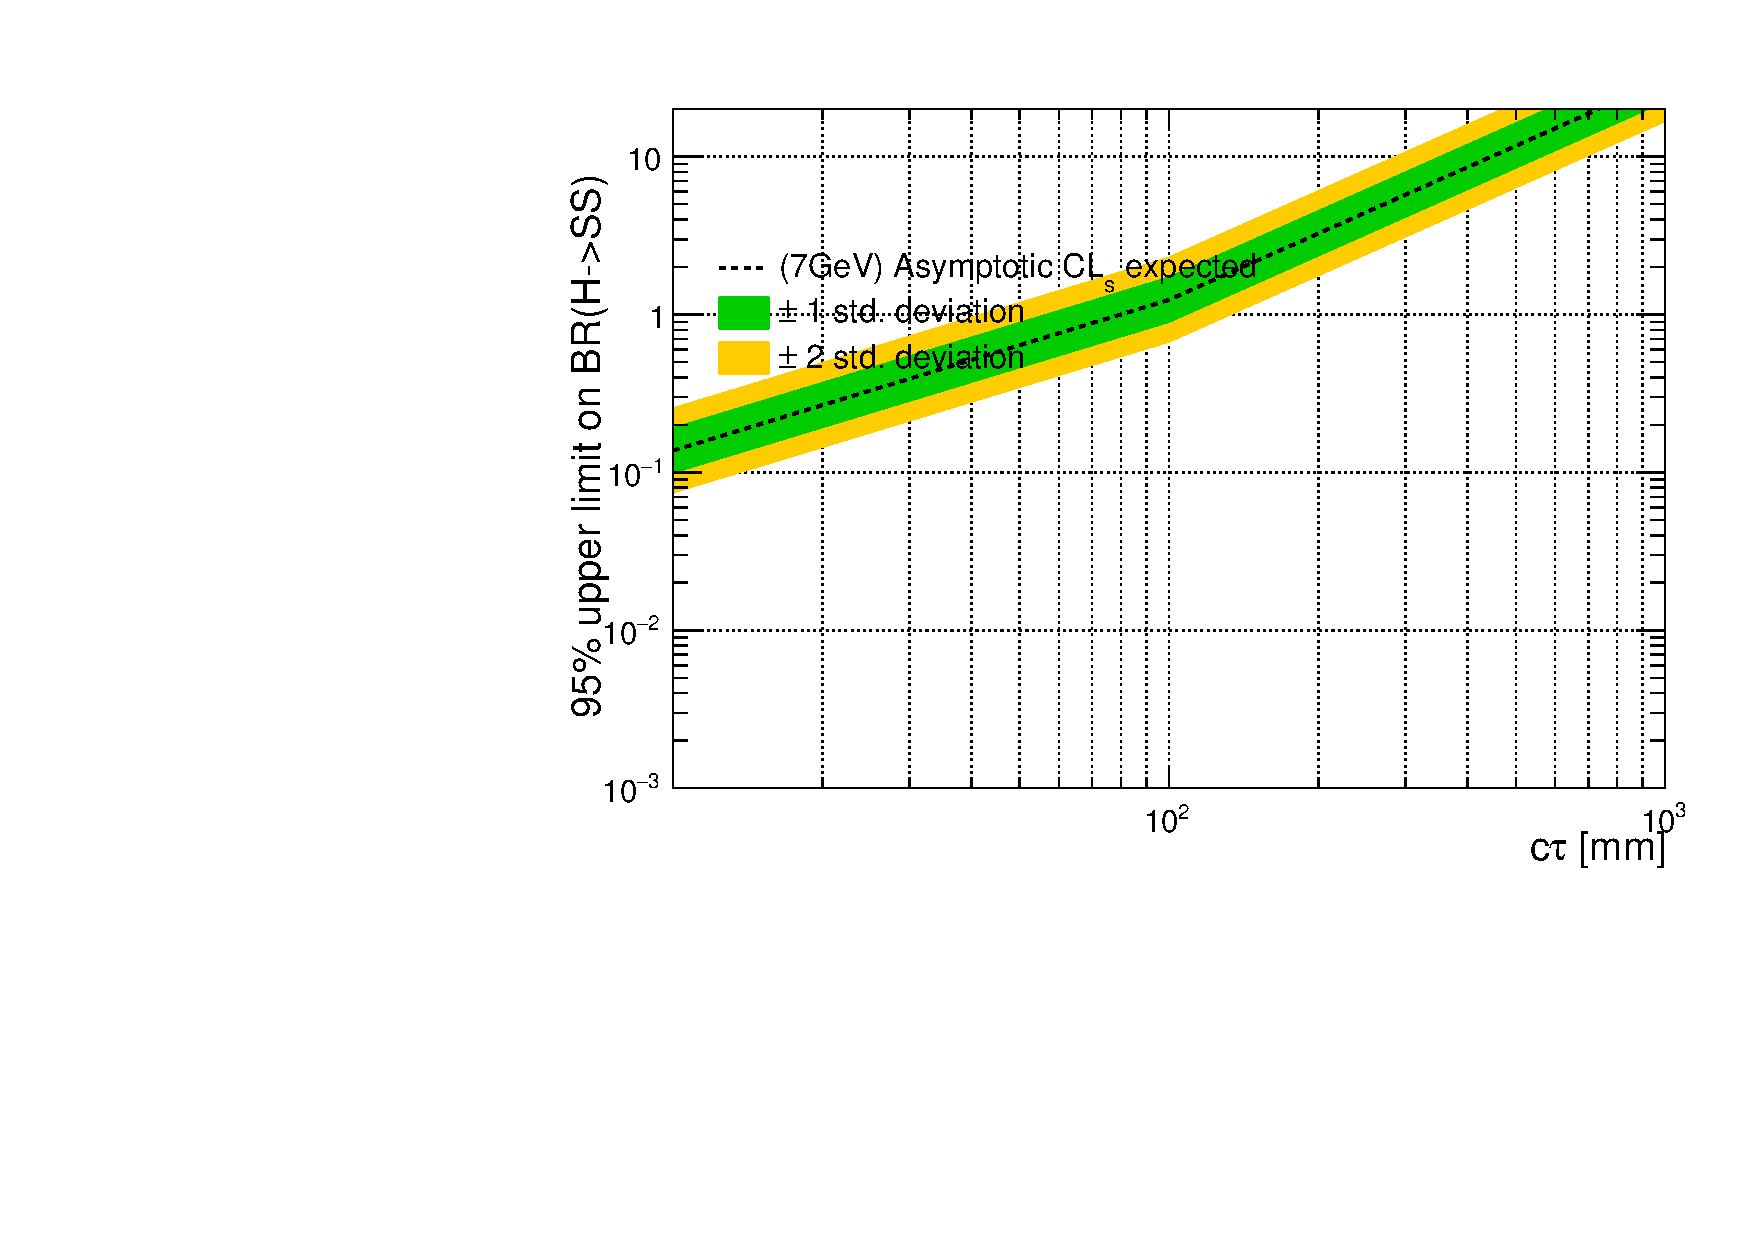
\includegraphics[width=0.48\linewidth]{figs/7GeVUpperLimit.pdf}
   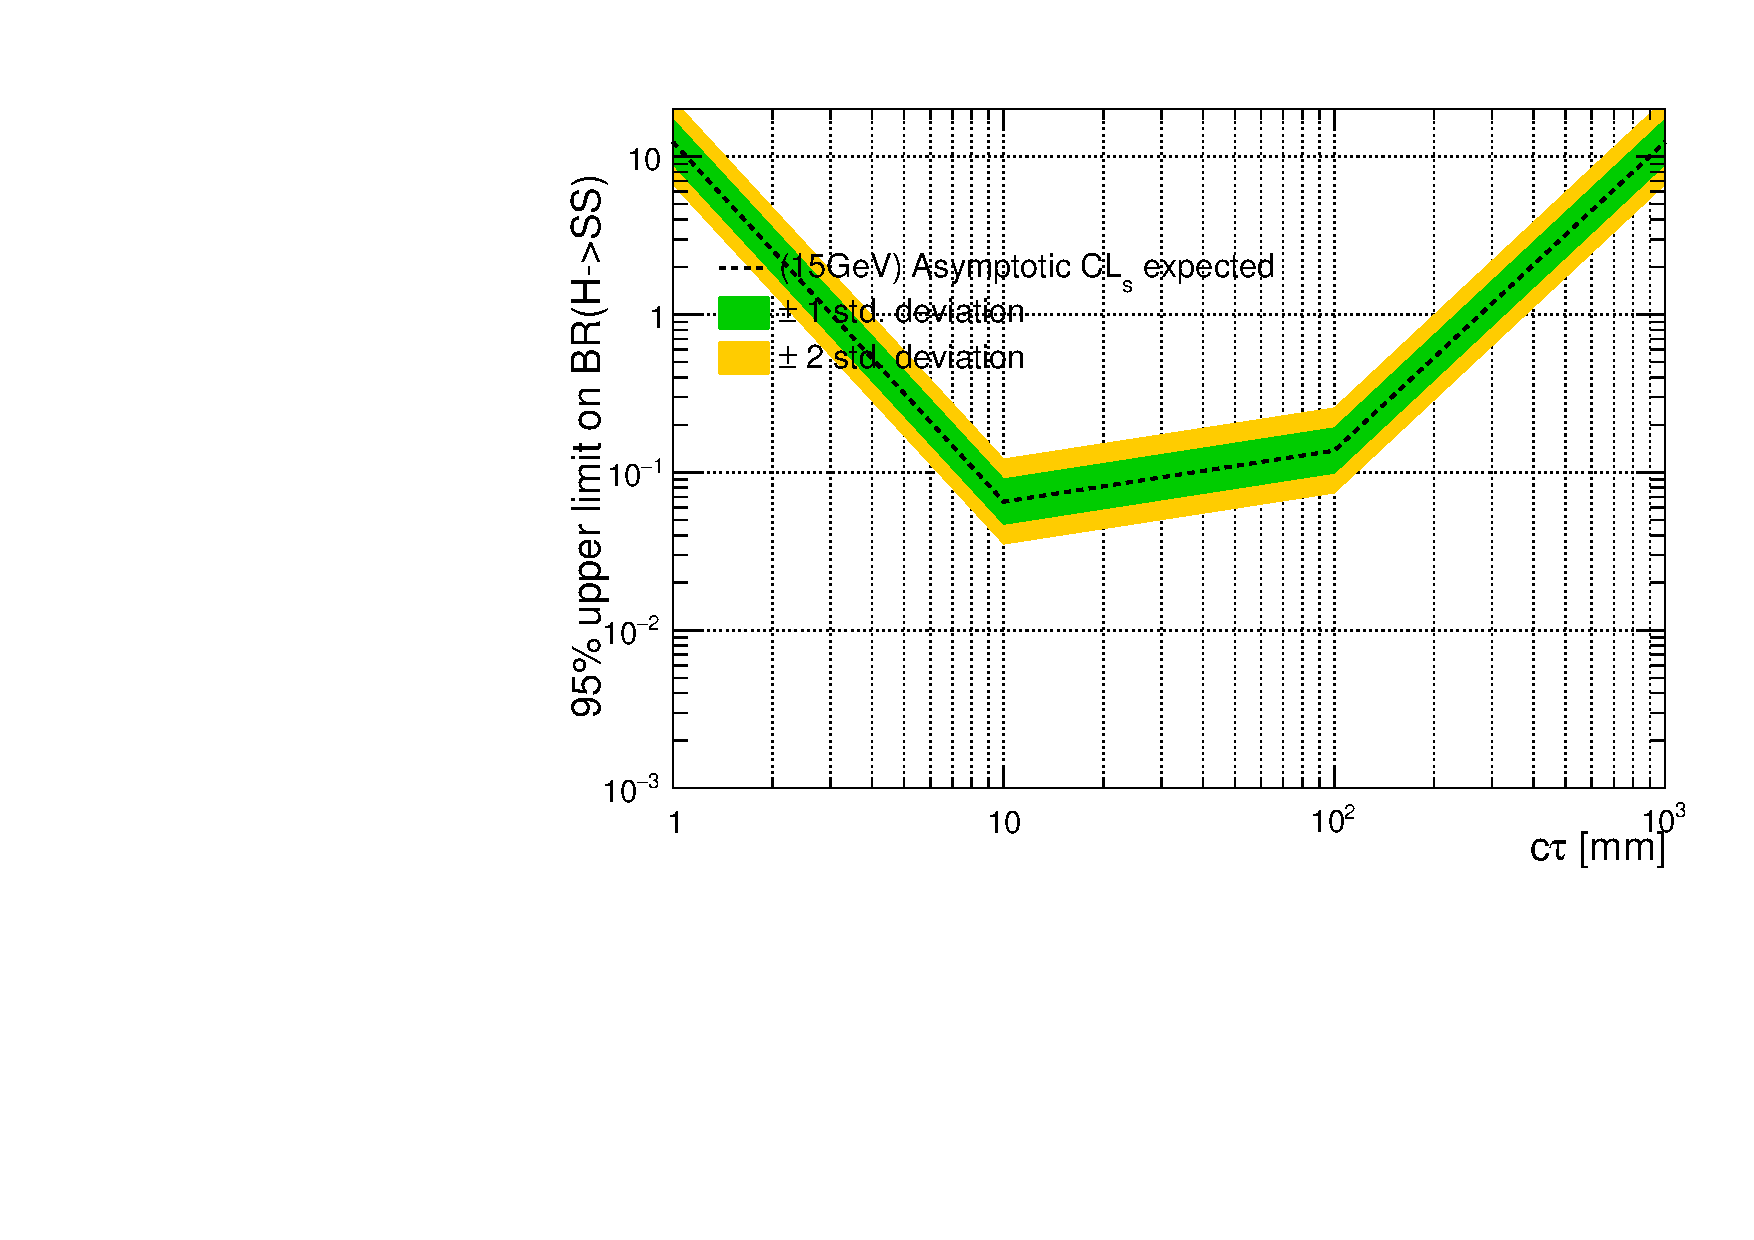
\includegraphics[width=0.48\linewidth]{figs/15GeVUpperLimit.pdf}
 \end{figure}
 \begin{figure}[h!]
   \caption{Current Preliminary limit plots}
   \label{fig:Limit2}
   \centering
   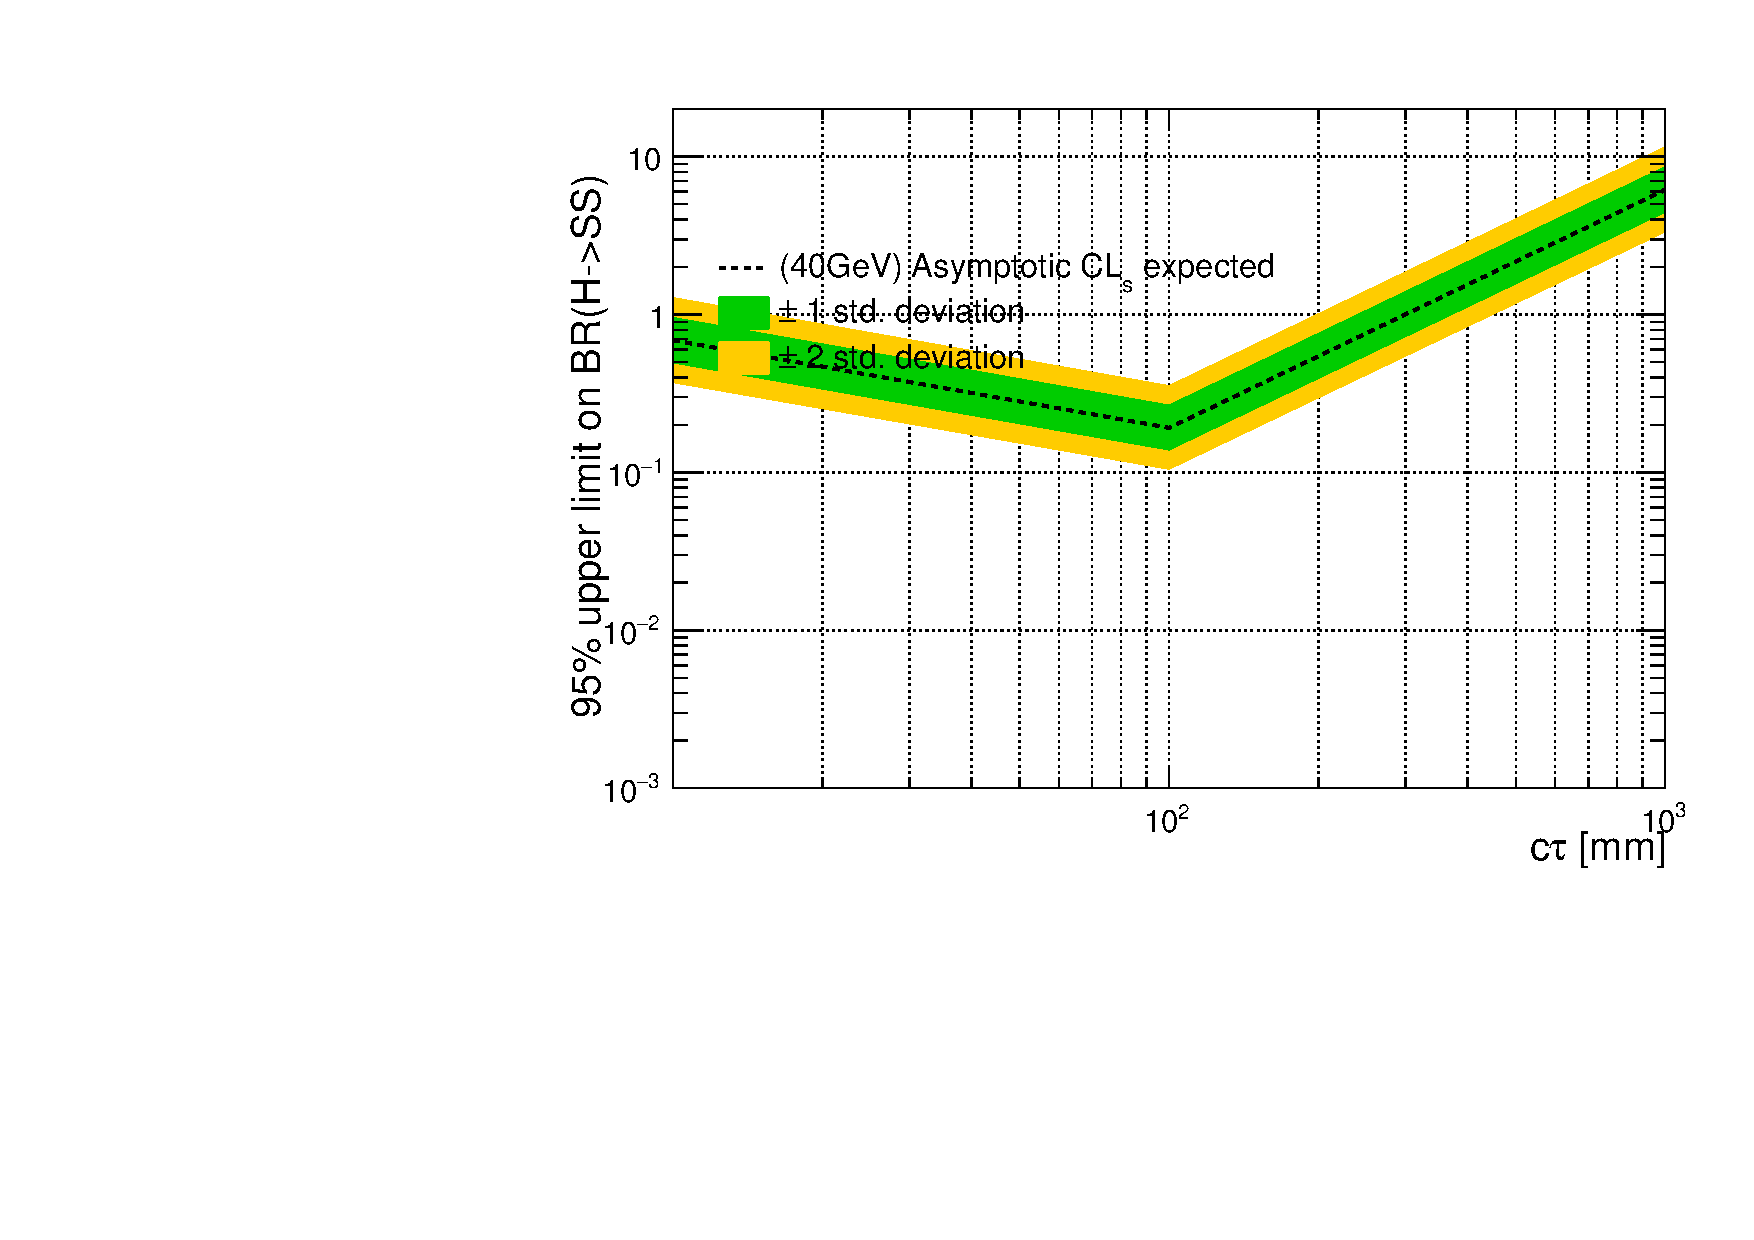
\includegraphics[width=0.48\linewidth]{figs/40GeVUpperLimit.pdf}
   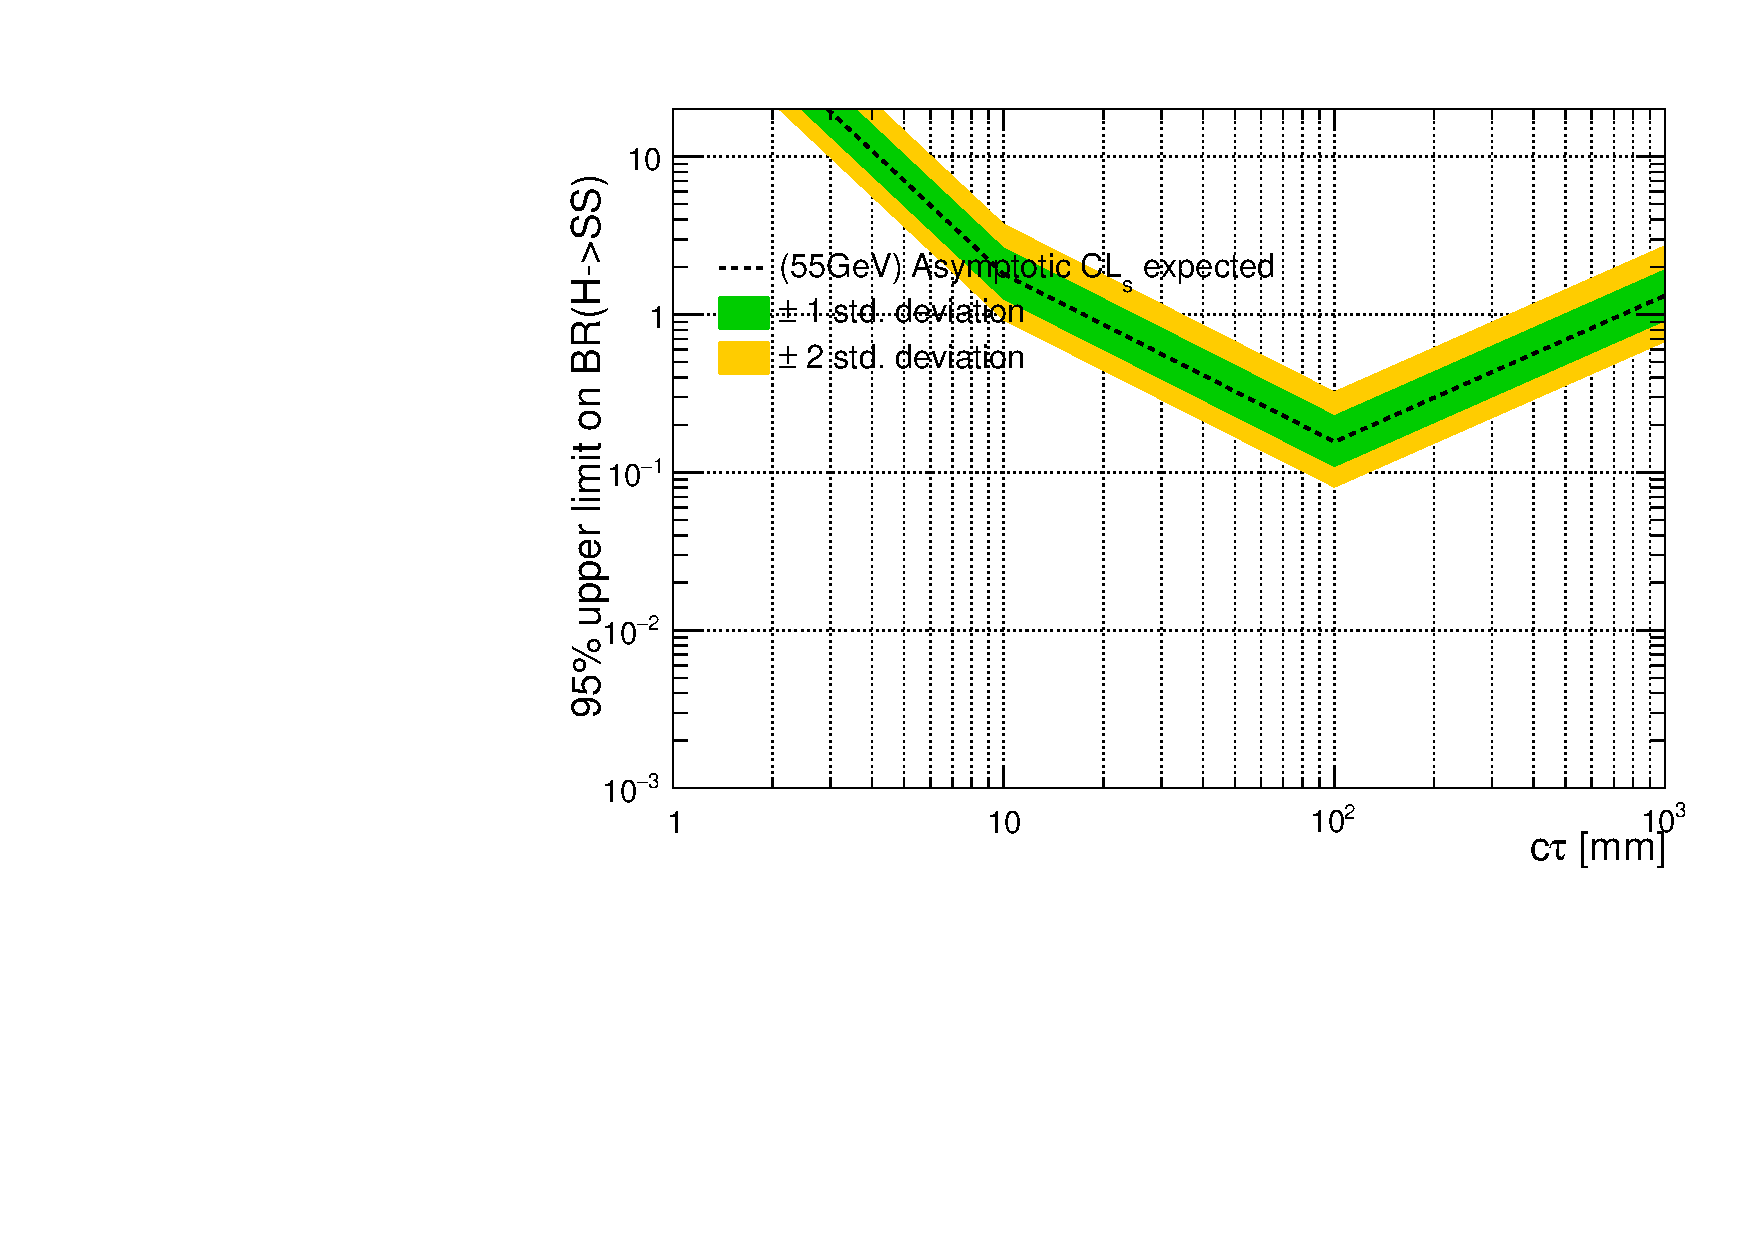
\includegraphics[width=0.48\linewidth]{figs/55GeVUpperLimit.pdf}
 \end{figure}
